\section{Correctness\label{section:inductive-correctness}}

Proving the correctness of our synthesis approach amounts to show that the synthesized system is consistent with both the scenarios and all domain knowledge taken in input. We discuss proof arguments for the different algorithm settings, starting with the simplest case of RPNI-based synthesis and gradually integrating features such as scenario questions and injection of domain knowledge.

\begin{figure}\centering
\scalebox{.65}{
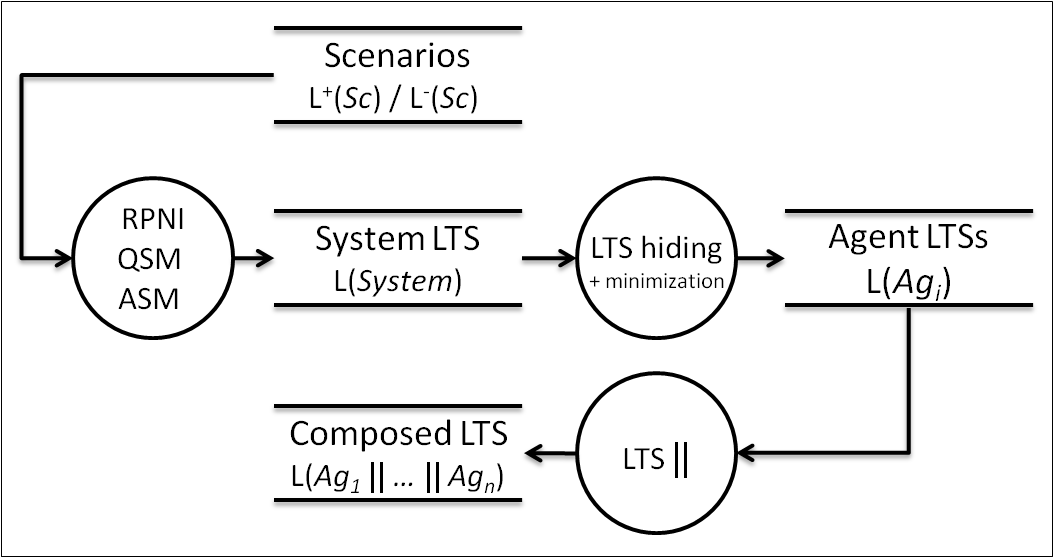
\includegraphics[trim=3mm 3mm 3mm 3mm, clip]{src/4-inductive/images/synthesis-flow-model}}
\caption{Inductive synthesis steps and products.\label{figure:synthesis-flow-model}} 
\end{figure}

Fig.~\ref{figure:synthesis-flow-model} summarizes our approach by showing used algorithms together with their input/output in terms of behavior models and associated languages. 
\begin{itemize}
\item From scenarios, a system LTS is inferred using either RPNI, QSM or ASM. 
\item LTS hiding and minimization is then used to obtain a canonical state machine for each agent. 
\item From the system view point, the result of our synthesis approach is precisely captured by the composition of those state machines.
\end{itemize}

In this figure and in the following discussion,
\begin{itemize}
\item $Sc = (S^+,S^-)$ denotes the input scenario collection; its positive and negative languages are denoted by $\mathcal{L}^+(Sc)$ and $\mathcal{L}^-(Sc)$, respectively.
\item $\mathcal{L}(\me{System})$ denotes the language captured by the inferred system LTS.
\item $\mathcal{L}(Ag)$ denotes the language of an arbitrary agent $Ag$, as captured by its LTS state machine.
\item $\mathcal{L}(\agentscomposed)$ denotes the language captured by the LTS resulting of the composition of individual agent LTSs.
\end{itemize}

We first restrict our attention to the simplest, non-interactive, RPNI approach. Remember from Section~\ref{subsection:inductive-synthesis-statement} that the specification on our approach requires three conditions to hold on synthesized state machines:
\begin{itemize}
\item The \emph{structural consistency} condition requires input scenarios and synthesized agent state machines to agree on the respective agent interfaces.
\item The \emph{consistent agent view} condition requires each synthesized agent state machine to cover the positive behaviors along the corresponding timeline in the input scenarios.
\begin{align}
\mathcal{L}^+(Sc_{\downarrow Ag}) \subseteq \mathcal{L}(Ag)\mbox{~for each agent $Ag$}\label{proof:consistent-agent-view}
\end{align}
where $Sc_{\downarrow Ag}$ denotes the positive behaviors along $Ag$'s timeline in a scenario collection $Sc = (S^+, S^-)$:
\begin{align}
\mathcal{L}^+(Sc_{\downarrow Ag}) = \bigcup_{P \in S^+} \mathcal{L}(P_{\downarrow Ag})~~\cup~~\bigcup_{N \in S^{-}} \mathcal{L}^{+}(N_{\downarrow Ag})\label{proof:lemma-sc-projection}
\end{align}

This is a a slight generalization of the concept of agent traces along a single scenario timeline $M_{\downarrow Ag}$, introduced in Section~\ref{section:background-scenarios}. Observe that it takes both positive and negative scenarios into account.
\item The \emph{consistent system view} requires the system to cover all positive scenarios and reject all negative ones. 
\begin{align}
&\mathcal{L}^+(Sc) \subseteq \mathcal{L}(\agentscomposed)\label{proof:consistent-system-view-1}\\
&\mathcal{L}^-(Sc) \cap      \mathcal{L}(\agentscomposed) = \emptyset\label{proof:consistent-system-view-2}
\end{align}
\end{itemize}

Section~\ref{subsection:system-lts-consistency} briefly discusses the consistency of the inferred system LTS with the scenarios. This result is then used in Section~\ref{subsection:consistent-agent-view} to show that the decomposition step meets the ``structural consistency'' and the ``consistent agent view'' conditions. The ``consistent system view'' condition is further discussed in Section~\ref{subsection:consistent-system-view}. The discussion is pursued in the presence of scenario questions in Section~\ref{subsection:proof-with-scenario-questions} and with the injection of domain knowledge in Section~\ref{subsection:proof-with-domain-knowledge}. Section~\ref{subsection:correctness-of-asm} closes this section with a discussion about the correctness of ASM.

%%%

\subsection{Consistency of the system LTS\label{subsection:system-lts-consistency}}

RPNI provides a guarantee that the system LTS covers all positive scenarios and rejects all negative ones. In other words, the following conditions hold:
\begin{align}
&\mathcal{L}^+(Sc) \subseteq \mathcal{L}(System)\label{proof:consistent-system-lts-1}\\
&\mathcal{L}^-(Sc) \cap      \mathcal{L}(System) = \emptyset\label{proof:consistent-system-lts-2}
\end{align}
where \emph{System} denotes the system LTS inferred from the scenario collection~\emph{Sc}.

This can be proven by induction. Roughly, 
\begin{itemize}
\item A precondition states that input scenarios are consistent. Therefore, conditions (\ref{proof:consistent-system-lts-1}) and (\ref{proof:consistent-system-lts-2}) initially hold on the PTA.
\item Those conditions hold for any quotient automata considered as intermediate solution of the induction process. On one side, quotient automata may only generalize the positive language (see Definition~\ref{definition:quotient-automaton}). On the other side, quotient automata are automatically discarded when inconsistent with the negative scenarios.
\end{itemize}

A detailed proof of RPNI and its convergence can be found in~\cite{Oncina:1993} in the more general case of transducer learning.

%%%

\subsection{Structural consistency and consistent agent view\label{subsection:consistent-agent-view}}

Given the consistency of the system LTS with the positive and negative scenarios, the decomposition step guarantees that the \emph{structural consistency} and the \emph{consistent agent view} both hold.

Structural consistency only requires the LTS hiding step to make use of adequate agent alphabets, as induced from the scenarios themselves or given by a (consistent) structural model. We do not discuss it further. 

For each agent $Ag$, the ``consistent agent view'' condition (\ref{proof:consistent-agent-view}) can be derived from (\ref{proof:consistent-system-view-1}) using the following properties and definitions:
\begin{align}
&\mathcal{L}(X) \subseteq \mathcal{L}(Y) \implies \mathcal{L}(X \setminus I) \subseteq \mathcal{L}(Y \setminus I) \label{proof-agent-consistency-1}\\
&\mathcal{L}^+(Sc_{\downarrow Ag}) = \mathcal{L}^+(Sc \setminus \Sigma_{Ag}^c)\label{proof-agent-consistency-2}\\
&\mathcal{L}(Ag) = \mathcal{L}(System \setminus \Sigma_{Ag}^c)\label{proof-agent-consistency-3}
\end{align}
where $\Sigma_{Ag}^c$ denotes the set of all system events excluding those of $Ag$'s interface.
\begin{itemize}
\item (\ref{proof-agent-consistency-1}) states that behavior inclusion is preserved under LTS hiding; this property follows from material in Section~\ref{subsection:lts-hiding}. 
\item (\ref{proof-agent-consistency-2}) rewrites the left term of (\ref{proof:consistent-agent-view}) in terms of hiding of scenario behaviors\footnote{using an abuse of notation as the hiding operator is defined on LTS, not on scenarios collections.}. It can be derived from (\ref{proof:lemma-sc-projection}) and the definition of $M_{\downarrow Ag}$ (see Section~\ref{subsection:background-positive-scenarios}). 
\item (\ref{proof-agent-consistency-3}) follows from the definition (\ref{definition:decomposition-step}) of decomposition step itself (see Section~\ref{subsection:inductive-synthesis-approach}). 
\end{itemize}

Given that condition (\ref{proof:consistent-system-lts-1}) holds, the following condition is established thanks to (\ref{proof-agent-consistency-1})
\begin{align}
&\mathcal{L}^+(Sc \setminus \Sigma_{Ag}^c) \subseteq \mathcal{L}(System \setminus \Sigma_{Ag}^c)\label{proof:consistent-agent-view-milestone}
\end{align}

The ``consistent agent view'' condition (\ref{proof:consistent-agent-view}) is established by substituing the right terms of (\ref{proof-agent-consistency-2}) and (\ref{proof-agent-consistency-3}) in (\ref{proof:consistent-agent-view-milestone}).

%%%

\subsection{Consistent system view: the problem of implied scenarios\label{subsection:consistent-system-view}}

The positive part of the ``consistent system view'' condition (\ref{proof:consistent-system-view-1}) follows from two main properties of our approach:
\begin{itemize}
\item The synthesized system LTS covers all positive scenario behaviors, as guaranteed by (\ref{proof:consistent-system-lts-1})
\begin{align*}
&\mathcal{L}^+(Sc) \subseteq \mathcal{L}(System)
\end{align*}
\item Projecting the system LTS on agent alphabets and recomposing their LTS afterwards cannot restrict behaviors:
\begin{align*}
&\mathcal{L}(\mbox{System}) \subseteq \mathcal{L}(\agentscomposed)
\end{align*}
This latter condition can be derived from the definition of agent languages (\ref{proof-agent-consistency-3}) and properties of LTS hiding and composition operators (see Section~\ref{section:background-state-machines}).
\end{itemize} 

The negative part of the ``consistent system view'' condition (\ref{proof:consistent-system-view-2}) requires the composed system to exclude all negative scenarios. Due to the potential presence of implied scenarios, our approach only guarantees a weaker condition (\ref{proof:consistent-system-lts-2}), namely,
\begin{align*}
&\mathcal{L}^-(Sc) \cap \mathcal{L}(\mbox{System}) = \emptyset
\end{align*}

In other words, the induction algorithm ensures that the \emph{system LTS} excludes all negative scenarios~\cite{Oncina:1993}. This property can however be lost after the decomposition and recomposition steps.

The reason has to be found in the possible occurence of so-called \emph{implied scenarios}. Remember from Section~\ref{subsection:background-hmsc} that implied scenarios may appear when a system is specified globally while implemented component-wise ~\cite{Alur:2000, Uchitel:2004}. In our case, the set of implied scenarios is precisely defined as:
\begin{align*}
\mathcal{L}(\agentscomposed) \setminus \mathcal{L}(\mbox{System})
\end{align*}

When this language is not empty, implied scenarios denote system behaviors that the system LTS does not accept but which are exhibited by the composition of agent LTSs. Implied scenarios appear when, once distributed, the agents lack monitoring abilities to restrict their behavior so as to precisely match the system LTS.

Not all implied scenarios are problematic in practice. In particular, it might happen that all implied scenarios denote desired system behaviors. In that case, the presence of implied scenarios is not problematic and may be seen as the result of a second generalization step due to the decomposition and recomposition of agent LTS. This second generalization step proves useful as it weakens the necessity of having a pure structurally complete scenario collection in the first place.

Negative implied scenarios, that is, counterexamples of desired behaviors, are more problematic. In particular, a behavior trace $t$ could be such that the following conditions hold:
\begin{align}
&t \in \mathcal{L}^-(Sc)\label{implied-1}\\
&t \notin \mathcal{L}(\mbox{System})\label{implied-2}\\
&t \in \mathcal{L}(\agentscomposed)\label{implied-3}
\end{align}
that is, (\ref{implied-1}) $t$ denotes a system behavior explicitly rejected through a negative scenario; it might be a question answered negatively; (\ref{implied-2}) $t$ is correctly rejected by the system LTS; (\ref{implied-3}) $t$ is still be exhibited by the composed system.

In such case, observe the ``consistent system view'' condition is not met as (\ref{proof:consistent-system-view-2}) does not hold. As with other scenario approaches, e.g. \cite{Alur:2000, Uchitel:2004}, our synthesis technique fails to guarantee a consistent system view between scenarios and state machines in presence of negative implied scenarios.

In order to detect such situations, the technique from \cite{Uchitel:2004} could be adapted to enumerate implied scenarios and submit them as additional scenario questions to the user (see Section~\ref{section:related-for-analysis-3}). 

Note that, fixing implied scenario problems requires rethinking the system decomposition into agents and/or refactoring their interfaces. In other words, the root cause of implied scenarios problems has to be found in the structural decomposition of the system, not in the particular technique used to infer state machines from scenarios. 

%%%

\subsection{Correctness in the presence of scenario questions\label{subsection:proof-with-scenario-questions}}

The specification of QSM has been strengthened in Section~\ref{section:lts-induction-from-mscs}. This strengthening required the synthesized system to be consistent with all scenario questions in addition to the initial scenario collection. 

Once a system LTS is inferred, correctness arguments for the \emph{structural consistency} and \emph{consistent agent view} conditions remain unchanged. The discussion about implied scenarios also takes place here. Therefore, we only discuss the consistency of the system LTS induced by QSM.

\begin{proof}
This can be proven by induction along the following lines (cfr. to Algo.~\ref{QSM}):
\begin{itemize}
\item The base case captures a QSM run where all scenario questions are answered positively. In such case, QSM roughly reduces to RPNI, for which conditions (\ref{proof:consistent-system-lts-1}) and (\ref{proof:consistent-system-lts-2}) about the consistency of the synthesized system LTS are known to hold \cite{Oncina:1993}.

For this particular run, we still need to prove that all scenario questions are accepted by the synthesized system LTS. Observe that when accepted (line 7), these scenarios are consistent with the current solution $A_{new}$ (line 4). The system LTS returned by QSM is a quotient automaton of $A_{new}$; Definition \ref{definition:quotient-automaton} therefore ensures that the system LTS accepts those scenarios as well.
\item Every time a scenario question is rejected by the oracle, the scenario collection is correctly extended (see line 9). Provided the oracle does not make classification errors, as required in preconditions, the scenario collection remains consistent. The recursive call on the extended scenario collection provides the inductive step (see line 10).
\end{itemize}
\end{proof}

%%%

\subsection{Consistency with goals and domain properties\label{subsection:proof-with-domain-knowledge}}

The consistency of the synthesized system LTS with available safety properties is captured by the following condition:
\begin{align}
&\mathcal{L}^-(G) \cap \mathcal{L}(\emph{System}) = \emptyset \mbox{~~for every safety property~G}\label{consistency-of-system-lts-with-goals}
\end{align}

This condition can be seen as the generalization of~(\ref{proof:consistent-system-lts-2}) which required the consistency of the synthesized system LTS with available negative scenarios.

Condition (\ref{consistency-of-system-lts-with-goals}) is proven by contradiction.
\begin{proof}
Let $G$ denote a safety property. Suppose the existence of a trace $s$ accepted by the system LTS while violating $G$, that is, $s \in \mathcal{L}(\me{System})$ and $s \in \mathcal{L}^-(G)$

A precondition of QSM requires input scenarios to be consistent with safety properties. The initial PTA solution $A_0$ does not generalize the positive scenario language; therefore $s \notin \mathcal{L}(A_0)$ and (\ref{consistency-of-system-lts-with-goals}) initially holds. 

By construction, there must exists a state pair $(q,q')$ considered for merging by QSM on a quotient automaton $A_i$ of the PTA, such that $s \notin \mathcal{L}(A_i)$ while $s \in \mathcal{L}(A_{i+1})$, where $A_{i+1}$ denotes the quotient automaton resulting from merging $q$ and $q'$ in $A_i$. 

We now prove that $q$ and $q'$ correspond to different states in the tester automaton of $G$ and have thus not been merged.

As $s$ is not accepted by $A_i$ but is accepted by $A_{i+1}$, there exists a suffix $w$ denoting a trace accepted from $q$ in $A_i$ whereas it is non-accepted from $q'$, or the converse. 

The tester automaton for $G$ is known to be deterministic, to have a complete transition function, and only one sink accepting state. As $s$ denotes a trace violating $G$, it reaches such accepting state in its tester. 

Let $t(q)$ and $t(q')$ denote the states of the tester corresponding to $q$ and $q'$ in the PTA, respectively.
\ldots
\end{proof}

%%%

\subsection{Correctness of ASM\label{subsection:correctness-of-asm}}

The correctness proof for ASM follows the same reasoning as the one presented for RPNI in Section~\ref{subsection:system-lts-consistency}.
\begin{itemize}
\item The input hMSC is required to be consistent with negative scenarios.
\item The initial solution automaton $A_0$ considered by ASM is returned by the \emph{Initialize} function. The latter implements the synthesis algorithm from \cite{Uchitel:2003} which does not generalize hMSC behaviors. Therefore, the consistency invariant \ref{XXX} initially holds for $A_0$.
\item The main induction loop is similar to the one of RPNI. It considers successive quotient automata, discarding those inconsistent with the negative scenarios.
\end{itemize}
